
\documentclass[sigconf,review, anonymous]{acmart}
\acmConference[ESEC/FSE 2019]{The 27th ACM Joint European Software Engineering Conference and Symposium on the Foundations of Software Engineering}{26--30 August, 2019}{Tallinn, Estonia}


\usepackage{expl3}
\expandafter\def\csname ver@l3regex.sty\endcsname{} 

\captionsetup[figure]{font=small}







\settopmatter{printacmref=false} % Removes citation information below abstract
\renewcommand\footnotetextcopyrightpermission[1]{} % removes footnote with conference information in first column
\pagestyle{plain}

\setcitestyle{square,sort,comma,numbers}
\usepackage{amssymb}% http://ctan.org/pkg/amssymb
\usepackage{pifont}% http://ctan.org/pkg/pifont
\settopmatter{printacmref=false}

\newcommand{\commentty}[1]{{\color{blue} \sf (TY: #1)}}
\newcommand{\commentlh}[1]{{\color{red} \sf (LH: #1)}}

\def\BibTeX{{\rm B\kern-.05em{\sc i\kern-.025em b}\kern-.08em
		T\kern-.1667em\lower.7ex\hbox{E}\kern-.125emX}}

\setcopyright{none} 

\begin{document}

	

	\title{Socio-Technical Aspects of package dependencies in software ecosystems}

	\author{Mehdi Golzadeh}
	\authornote{Both authors contributed equally to this research.}
	\email{mehdi.golzadeh@umons.ac.be}
	\orcid{0000-0003-1041-439X}
	\affiliation{%
	\institution{Software Engineering Lab, UMONS}
	\city{Mons, Belgium}
	\postcode{7000}
	}
	
	\newcommand*{\Scale}[2][4]{\scalebox{#1}{$#2$}}%
	\newcommand{\Tool}{ComAir\xspace}
	\newcommand{\ComBugs}{30\xspace}
	%\newcommand{\Code}[1]{\lstinline{#1}}
	%\newcommand{\comment}[1]{{}}
	
	
	
	
	
	\begin{abstract}
		I think here we dont need an abstract cause it is a two page abstract. but I dont know how should section it.
	\end{abstract}
	
	
	
	\maketitle
	
\section{Introduction}
\label{sec:intro}

Today's software development is increasingly relying on software package libraries distributed through open source software (OSS) package managers (such as Cargo, npm, Maven and CRAN). Rather than writing software from scratch, developers often choose to depend on existing software packages.
At the same time, collaborative online development platforms like GitHub make software development an inherently social phenomenon~\cite{DabbishSTH12,Mens2019IEEESW}.

The collection of packages distributed by a software package manager forms a \emph{socio-technical} dependency network. Packages depend on other packages that are required for installing and deploying them. Software developers are \emph{technically} contributing to these packages (e.g., by making commits, pull requests to the package's git repository). Software developers are also \emph{socially} active (e.g., by commenting on the commit and pull request activities).
%Do you think its better to move the issue reporting activity to the social activities?
The phenomenon of socio-technical congruence (a.k.a. Conway's law)~\cite{Conway1968, Herbsleb1999} assumes
that the package dependency network structure and the communication structure of its community of contributors are tightly interwoven. Very little research focuses on such socio-technical congruence at the ecosystem level~\cite{Palyart2018TSE}, or studies show the congruence evolves over time~\cite{Cataldo2008}.

My PhD research %started in June 2019, and
aims to empirically study, within evolving OSS %packaging 
ecosystems, the socio-technical congruence between package dependencies, the interaction patterns of package contributors and how this affects the health of the ecosystem. % As such, I aim to gain a better understanding of how this affects the health of the packaging ecosystem.
To do so %for package dependency networks of OSS package managers,
I will explore 3 research questions: 
%
% to find if there is some tendency or correlation between package dependency network and the  collaborator communication network:
%\noindent 
\textbf{RQ$_1$} \emph{How does the dependency network structure influence social activity?} %(E.g., are contributors more likely to be active in commenting on packages they depend on than on other packages?
%\noindent
 \textbf{RQ$_2$} \emph{How does the social activity of package contributors increase their likelihood to start/stop depending on this package?}
%\noindent
\textbf{RQ$_3$} \emph{How does the social activity of package contributors increase their likelihood to start/stop becoming technically active?}


In the first phase, I will focus on packages distributed through the Cargo package manager and developed on GitHub %, the biggest online collaborative development platform
%.
%I will focus on
by studying their \emph{technical} development activity (e.g., GitHub commits and pull requests% and issue reports
) and \emph{social} communication activity %(e.g., commit comments, pull request comments and issue comments through GitHub).
(e.g., commit comments and pull requests comments). 
%
Other %research questions, 
activity types and packaging 
ecosystems will be explored in a later phase, on the basis of the results obtained %for the Cargo case study
in the first phase. %These follow-up 
These questions will focus on the expected benefits that socio-technical congruence will have on the health of the ecosystem and its community, such as increased productivity, responsiveness, contributor intake and retention.
\section{Data Extraction and Analysis} 

The \textsf{libraries.io} monitoring service contains package metadata, including dependencies for 36 different package managers.
I have selected the Cargo package manager for the Rust programming language as a first case study. It was created in 2014, and most of its packages are developed on GitHub. 
Cargo is growing fast in number of packages, package releases, dependencies and contributors~\cite{Decan2019EMSE}. 
%By studying this package dependency network I hope to gain insights into how the ecosystem growth affects the socio-technical congruence over time and vice versa.

I used on a datadump of \textsf{libraries.io}~\cite{Katz2018} to extract the temporal evolution of Cargo's package dependency network. 
For each package, I extracted %metadata such as
 the package name, release number and date, maintainer, package dependencies and their versioning constraints. 
The dataset contained $+15K$ packages, $+66K$ package releases and $+48K$ dependency relations.
I retrieved the (optional) link to the corresponding development repositories and filtered out packages for which no GitHub repository was found (1,984 cases) %1984 = 1571 + 413 
or that corresponded to duplicate repository links (3,500 cases).
 % I also found that 1571 of records contain no repository address, 413 of them have repository address other than GitHub and 3500 of them contains duplicate repository address.
I downloaded the relevant historical socio-technical data from the remaining 9,954 GitHub repositories.
%TO DO: Mention here how big is the libraries.io dataset you used (after filtering): how many packages; how many package releases; how may package dependencies; how many github repositories}
This data includes all contributors and their role, the \emph{social} commenting activities they were involved in ($+904K$ comments separated into commit comments, pull request comments, pull request review comments and issue comments), and the \emph{technical} development activities they had conducted ($+942K$ commits, $+145K$ pull requests and $+266K$ issues).
%The downloaded metadata was also fairly big including 942183 commits, 145053 pull requests, 266033 issues, 90228 unique comments-contributor.
%It is worthwhile to mention that 
3,170 repositories had no comments, and comments follow the Pareto rule ($80\%$ of all comments belong to $<20\%$ of all repositories).
\section{ANALYSIS AND RESULTS}

To study the socio-technical congruence of Cargo, I started analysing its package dependency network and the associated technical and social (commenting) activities of its GitHub contributors.
%For this purpose I used Python notebooks and relied on existing data analytics and statistical libraries.
Focusing on the research questions of Section~\ref{sec:intro}, I report some very preliminary analysis below.
For now, the presented results are anecdotal and need to be complemented with proper statistical hypothesis testing, survival analysis and prediction modeling.

I started to investigate how the commenting activity of contributors to a package relates to the introduction of a package dependency.
To do so, I considered all packages for which a new dependency was added at some point in time, and analysed whether commenting activity could be observed \emph{before} or \emph{after} depending on those packages.
Figure~\ref{fig:fig1} summarises the results. One can observe that more commenting activity happens on package repositories after the creation of dependencies to those packages than before adding such dependencies. 
An important shift in behaviour can be observed around September 2017, where the commenting activity before starting to depend on packages is increasing and an inverse trend shift is observed for the commenting activity after starting to depend on packages. Why this trend shift occurs remains an open question for now.

\begin{figure}[thb]
\vspace{-0.3cm}
    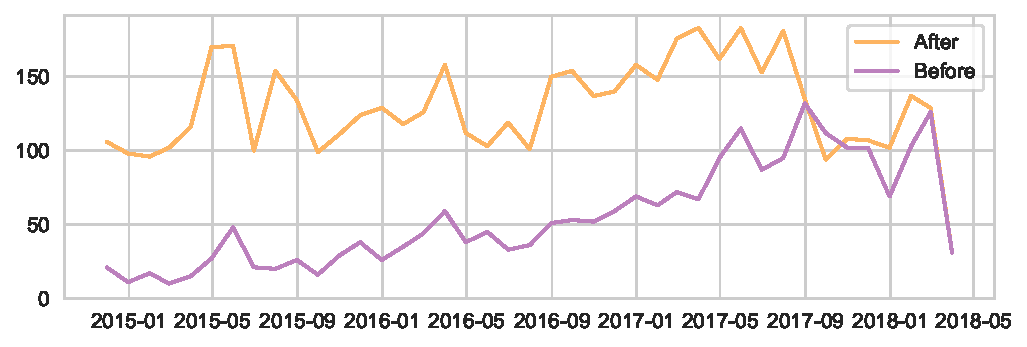
\includegraphics[width=0.9\columnwidth]{Photos/RQ21.pdf} 
    \caption{Commenting activity (number of comments) to package repositories before and after starting to depend on a package.}
    \label{fig:fig1}
\end{figure}

In order to assess which types of comments are more likely to lead to the introduction of new package dependencies, I analysed the proportion of comment types for all comments made in repositories of packages prior to the addition of a dependency to those packages. Figure~\ref{fig:fig2} presents these results. 
One can observe that, among the four types of comments considered (i.e., commit comments, issue comments, pull request comments and pull request review comments), the proportion of comments on pull requests and issue requests is considerably higher than for commit comments and review comments. I hypothesise that commenting on pull requests and issue requests for a package could serve as a good predictor for adding new dependencies to that package.

\begin{figure}[htb]
    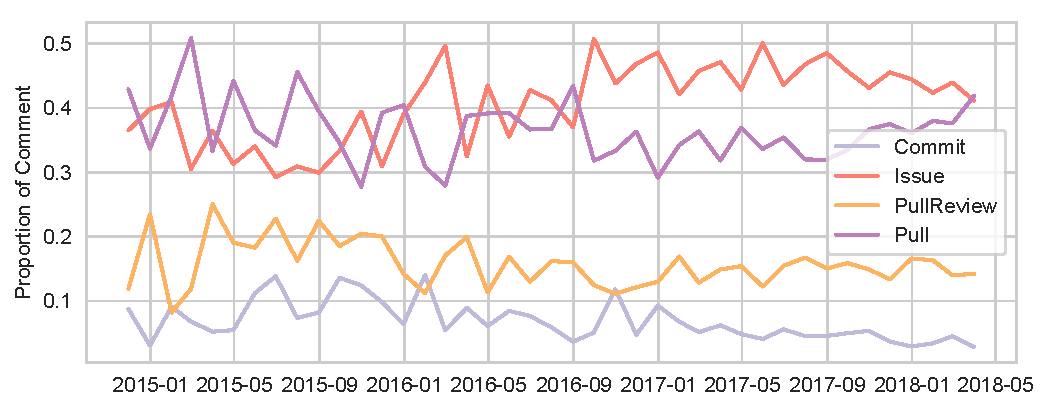
\includegraphics[width=0.9\columnwidth]{Photos/RQ22.pdf} 
    \caption{Proportion of comment types made in the repositories of packages before starting to depend on that package.}
    \label{fig:fig2}
\end{figure}

I also started to investigate whether social (i.e., commenting) activity on a package repository increases the likelihood to become technically active on that repository (i.e., submitting commits or pull requests). 
Figure~\ref{fig:fig3} presents some preliminary results. Considering the four different types of commenting activity, one can observe that issue comments are more likely to result in becoming technically active on a package repository.

\begin{figure}[thb]
    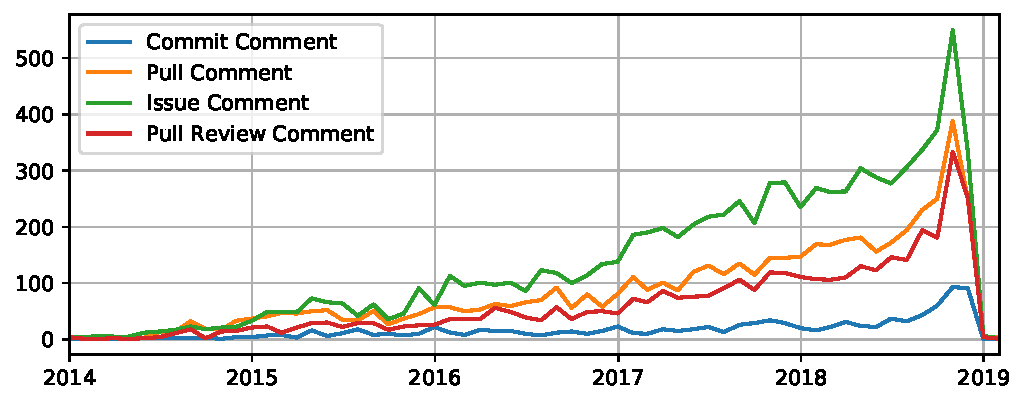
\includegraphics[width=0.9\columnwidth]{Photos/RQ3.pdf} 
    \caption{Number of comments (broken down by comment type) before starting  to technically contribute to a package.}
    \label{fig:fig3}
\end{figure}



	
	\bibliographystyle{ACM-Reference-Format}
	\bibliography{biblio.bib}



\end{document}

